%%%%%%%%%%%%%%%%%%%%%%%%%%%%%%%%%%%%%%%%%%%%%%%%%%%%%%%%%%%%%%%%%%%%%%%%
\chapter{Context}
%%%%%%%%%%%%%%%%%%%%%%%%%%%%%%%%%%%%%%%%%%%%%%%%%%%%%%%%%%%%%%%%%%%%%%%%

\begin{center}
  \begin{minipage}{0.5\textwidth}
    \begin{small}
      Hoofdstuk 2 besteedt aandacht aan de historie van de gesynthetiseerde stem en de hedendaags aanwezige technieken en initiatieven tot het realiseren van een menselijke stem met een eigen karakter. Het hoofdstuk wordt afgesloten met een afweging ten aanzien van de tegenwoordige initiatieven en de ontwikkelrichting van Prolody B.V.
    \end{small}
  \end{minipage}
  \vspace{0.5cm}
\end{center}

\noindent ...

%%%%%%%%%%%%%%%%%%%%%%%%%%%%%%%%%%%%%%%%%%%%%%%%%%%%%%%%%%%%%%%%%%%%%%%%
\section{Inleiding}
%%%%%%%%%%%%%%%%%%%%%%%%%%%%%%%%%%%%%%%%%%%%%%%%%%%%%%%%%%%%%%%%%%%%%%%%

Spraak synthese is de kunstmatige reproductie van menselijke spraak. Computer systemen die voor dit doeleinde worden gebruikt, worden ook wel spraakcomputers, spraaksynthesizers of een text-to-speech (TTS) systeem genoemd. Deze systemen zijn ontwikkeld voor de translatie van zowel fonetische als natuurlijke taal naar een audio representatie. De kwaliteit van een spraaksynthese systeem wordt doorgaans geëvalueerd op basis van verstaanbaarheid en de similariteit met de menselijke stem. In dit hoofdstuk worden een aantal technieken uiteengezet voor het synthetiseren van menselijke spraak.

\begin{figure}[]
    \centering
    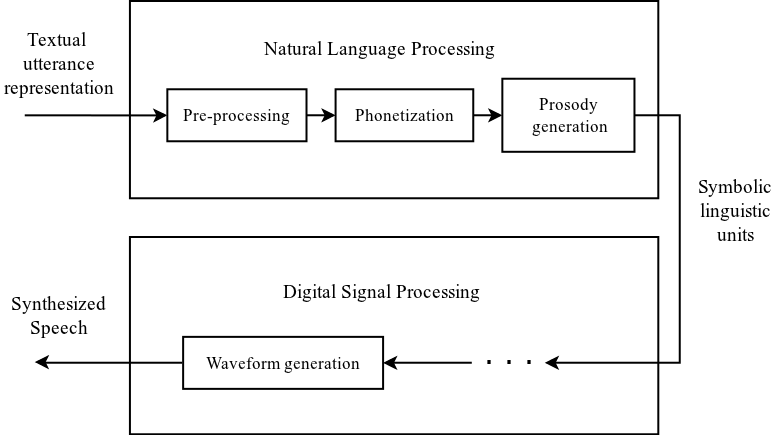
\includegraphics[width=0.5\textwidth]{figures/tts_system.png}
    \caption{Text-to-speech model \cite{speect}}
    \label{fig:tts}
\end{figure}

%%%%%%%%%%%%%%%%%%%%%%%%%%%%%%%%%%%%%%%%%%%%%%%%%%%%%%%%%%%%%%%%%%%%%%%%
\section{Probleemstelling}
%%%%%%%%%%%%%%%%%%%%%%%%%%%%%%%%%%%%%%%%%%%%%%%%%%%%%%%%%%%%%%%%%%%%%%%%

Vaak wordt gedacht dat het probleem van geschreven tekst vertalen naar spraak een probleem van 'omgekeerde spraakherkenning' is: huidige spraakherkenningssystemen worden als succesvol beschouwd als die opgenomen spraak kan vertalen naar de sequentie van woorden die zijn gezegd, dus men zou denken dat een TTS synthesizer begint bij de woorden in de tekst, die elk vertaalt naar een audio representatie, en de aparte resultaten aan elkaar hecht. Echter, het correct uitspreken van woorden is maar een onderdeel van spraak. Om een natuurlijke stem en een goede interpretatie van het gezegde te bewerkstelligen, moeten sommige woorden worden benadrukt en andere minder; een zin wordt op een betekenisvolle manier gefraseerd; er moet een gepaste contour van de $F_0$ (fundamentele) frequentie worden gekozen (de melodische contour in de stem), et cetera.

De moeilijkheid van de vertaalslag van tekst naar spraak, is het gebrek aan veel aspecten van informatie die van belang zijn voor spraak. Weliswaar representeert een zin alle woorden om de betekenis duidelijk te maken, maar het specificeert de frasering van een zin maar gedeeltelijk (door middel van bijvoorbeeld punctuatie), het specificeert niet de meer en minder benadrukte woorden en het geeft geen informatie over de intonatie of stemkwaliteit van een woord of frase.

TTS wordt vaak verdeeld in twee sub-problemen. Het eerste probleem adresseert de vertaling van tekst - een eigenlijk imperfecte representatie van taal zoals eerder aangegeven - in een linguïstieke vorm. Deze vorm bevat informatie over de fonemen die moeten worden geproduceerd, de duur en locaties van pauzeringen en de $F_0$ contour die moet worden gebruikt. Het tweede probleem adresseert de eigenlijke synthese van spraak. Het neemt de informatie uit het eerste probleem en vertaalt die naar een geluidsgolf.

Het eerste probleem, de tekst en linguïstieke analyse, wordt als volgt opgedeeld:
\begin{itemize}
    \item \textit{Tekst voorverwerking}: de detectie van het einde van de zin, tekst normalisatie (het volledig uitschrijven van nummers en afkortingen) en een grammaticale analyse, zoals het indelen van woorden in de bijbehorende, lexicale categorie (POS-tagging).
    \item \textit{Accentueren}: het aangeven van de nadruk die moet worden gelegd op bepaalde woorden.
    \item \textit{Uitspraak van woorden}: waarbij gelet wordt op de uitspraak van eigennamen, maar ook de desambiguatie van homoniemen \footnote{Een homoniem is een zelfstandig woord dat eenzelfde uitspraak heeft en tot eenzelfde woordsoort behoort, maar twee of meerdere geheel andere betekenissen heeft.}
    \item \textit{Fraseringen}: het fraseren van de zin door middel van intonatie.
    \item \textit{$F_0$ contour berekening}: waarbij een passende, melodische contour van de zin wordt berekend.
\end{itemize}

Het tweede probleem van spraak synthese wordt opgedeeld in twee delen:
\begin{itemize}
    \item de synthese van de spraak waveforms gegeven de gegenereerde, foneme delen in de eerste probleemstelling;
    \item de selectie en samenvoeging van zinsdelen gegeven de spraak waveforms.
\end{itemize}

%%%%%%%%%%%%%%%%%%%%%%%%%%%%%%%%%%%%%%%%%%%%%%%%%%%%%%%%%%%%%%%%%%%%%%%%
\section{Gesynthetiseerde stem}
%%%%%%%%%%%%%%%%%%%%%%%%%%%%%%%%%%%%%%%%%%%%%%%%%%%%%%%%%%%%%%%%%%%%%%%%

Text-to-speech synthese kent al een lange historie, beginnend bij Dudley's 'Voder' dat werd ontwikkeld bij Bell Laboratories en werd gedemonstreerd bij de World Fair in 1939 \cite{voder}. Een mens bestuurde de 10 bandpass filters van de 'Voder' om menselijke spraak te genereren. Pas vanaf de jaren '60 worden er systemen geïntroduceerd die automatisch spraak kunnen genereren op basis van linguïstieke representaties (zoals fonetische of tekstuele input). De twee belangrijkste technieken voor het synthetiseren van spraak waveforms zijn formantsynthese en concatinerende synthese (concatenative synthesis).

\subsection{Formantsynthese}
De eerste vorm van digitale spraaksynthese werd gerealiseerd met formantsynthese. Een formant is een smalle, piekende spectrale vorm die een oorsprong vindt in de resonantie van het menselijke spraakkanaal. Bij formantsynthese wordt gebruik gemaakt van additieve synthese en akoestieke modellering om spraak te genereren. Hierbij worden dus geen menselijke samples gebruikt.

\subsection{Concatenative synthesis}
Deze synthesetechniek synthetiseert geluid door middel van digitale, (korte) geluidssamples in een grote database slim te selecteren en samen te voegen (ook wel \textit{units} genoemd).

\subsubsection{Unit selection synthesis}
Een spraak synthesizer gebaseerd op concatenative synthesis gebruikt stukken natuurlijke spraak als bouwstenen om een arbritraire, nieuwe zin van spraak te reconstrueren \cite{nuance}. Een database van spraak \textit{units} is gemaakt met opnames van spraak. Door gebruik te maken van echte spraak worden een aantal karakteristieken van de stemacteur behouden. Een voordeel van \textit{Unit selection synthesis} is, dat wanneer er juiste \textit{units} worden gekozen, er een realistische stem met ook articulatie effecten ontstaat. Een ander voordeel is dat het een relatief eenvoudig systeem is, er hoeft weinig aandacht besteed te worden aan articulatie en synthese omdat er alleen gebruik wordt gemaakt van echte spraak \textit{units}.

In \textit{Unit selection synthesis} systemen wordt in een database gezocht naar foniemen die in dezelfde context als de \textit{target} foniemen voorkomen. Er wordt een \textit{penalty} voor het matchen van de gekozen foniem en de context gecaculeerd. Dit wordt gedaan door het verschil van de naburige foniemen in de \textit{target} en de naburige foniemen in de database te berekenen. De \textit{unit waveforms} van de \textit{target} worden daarna aan elkaar gezet (concatanation) door \textit{Pitch Synchronous Overlap and Add} (PSOLA) tussen aaneengesloten foniemen. Het algoritme past niet de prosodie aan, maar gebruikt dezelfde lengte, intonatie en articulatie van de foniem in de database. Het gebrek aan een goede, \textit{prosodic target} is een van de grootste tekortkomingen in dit systeem.

Om de ontwikkeling van een spraak \textit{unit} database te versnellen, zijn er automatische synthese \textit{unit} generation systemen ontwikkeld \cite{nakajima1994automatic}. Hierbij wordt de inventaris van spraak \textit{units} automatisch geannoteerd door middel van een al geannoteerde database (spraak waarvan de tekst al is getranscribeerd).


\subsubsection{Diphone synthesis}
ne popular unit is the diphone, which consists of the transition from the center of one phoneme to the center of the following one. This model helps to capture transitional information between phonemes. A complete set of diphones would number approximately 1600, since there

are approximately (40) possible combinations of phoneme pairs. Diphone speech synthesis thus requires only a mod erate amount of storage. One disadvantage of diphones is that they lead to a large number of concatenation points (one per phoneme), so that heavy reliance is placed upon an efficient Smoothing algorithm, preferably in combination with a diphone boundary optimization. Traditional diphone synthesizers, such as the TTS3000 of Lernout & Hauspie Speech and Language Products N.V., use only one candidate speech unit per diphone. Due to the limited prosodic vari ability, pitch and duration manipulation techniques are needed to synthesize speech messages. In addition, diphones synthesis does not always result in good output speech quality.



%%%%%%%%%%%%%%%%%%%%%%%%%%%%%%%%%%%%%%%%%%%%%%%%%%%%%%%%%%%%%%%%%%%%%%%%
\section{Hedendaagse technieken}
%%%%%%%%%%%%%%%%%%%%%%%%%%%%%%%%%%%%%%%%%%%%%%%%%%%%%%%%%%%%%%%%%%%%%%%%

\subsection{WaveNet}
WaveNet is een neuraal netwerk voor het genereren van audio waveforms \cite{45774}. Dit model is volledig probabilistisch en zelfvoorspellend, waarbij er een kansdistributie wordt berekend voor elk audio sample, geconditioneerd op alle vorige. Wanneer het wordt gebruikt in een tekst-to-speech toepassing, heeft het een state-of-the-art prestatie waarbij mensen het als significant beter en realistischer beoordelen dan de beste concatenative synthese systemen \footnote{\url{https://deepmind.com/blog/wavenet-generative-model-raw-audio}}. WaveNet kan ook worden gebruikt voor het herkennen van foniemen, voor bijvoorbeeld gebruik in concatenative synthesis.

WaveNet is ontwikkeld door DeepMind en ligt ten grondslag aan alle nieuwe text-to-speech systemen van Google die onder andere worden gebruikt in de Google Assistant \footnote{\url{https://cloud.google.com/text-to-speech/docs/wavenet}}.




\subsection{Tacotron}

\cite{Wang2017TacotronTE}
A text-to-speech synthesis system typically consists of multiple stages, such as a text analysis frontend, an acoustic model and an audio synthesis module. Building these components often requires extensive domain expertise and may contain brittle design choices. In this paper, we present Tacotron, an end-to-end generative text-to-speech model that synthesizes speech directly from characters. Given <text, audio> pairs, the model can be trained completely from scratch with random initialization. We present several key techniques to make the sequence-to-sequence framework perform well for this challenging task. Tacotron achieves a 3.82 subjective 5-scale mean opinion score on US English, outperforming a production parametric system in terms of naturalness. In addition, since Tacotron generates speech at the frame level, it's substantially faster than sample-level autoregressive methods. 


or machine translation (Wu et al., 2016),  TTS outputs are continuous,  and output sequences areusually much longer than those of the input. These attributes cause prediction errors to accumulatequickly.   In this paper,  we propose Tacotron,  an end-to-end generative TTS model based on thesequence-to-sequence (seq2seq) (Sutskever et al., 2014) with attention paradigm (Bahdanau et al.,2014).  Our model takes characters as input and outputs raw spectrogram, using several techniquesto improve the capability of a vanilla seq2seq model.   Given<text,  audio>pairs,  Tacotron canbe trained completely from scratch with random initialization.  It does not require phoneme-levelalignment, so it can easily scale to using large amounts of acoustic data with transcripts.  With asimple waveform synthesis technique, Tacotron produces a 3.82 mean opinion score (MOS) on anUS English eval set, outperforming a production parametric system in terms of naturalness1.


\subsection{Deep Voice}
\footnote{\url{https://r9y9.github.io/deepvoice3_pytorch/}}
We present Deep Voice 3, a fully-convolutional attention-based neural text-to-speech (TTS) system. Deep Voice 3 matches state-of-the-art neural speech synthesis systems in naturalness while training ten times faster. We scale Deep Voice 3 to data set sizes unprecedented for TTS, training on more than eight hundred hours of audio from over two thousand speakers. In addition, we identify common error modes of attention-based speech synthesis networks, demonstrate how to mitigate them, and compare several different waveform synthesis methods. We also describe how to scale inference to ten million queries per day on one single-GPU server. 


BAIDU \cite{Arik2017DeepVR}.
We present Deep Voice, a production-quality text-to-speech system constructed entirely from deep neural networks. Deep Voice lays the groundwork for truly end-to-end neural speech synthesis. The system comprises five major building blocks: a segmentation model for locating phoneme boundaries, a grapheme-to-phoneme conversion model, a phoneme duration prediction model, a fundamental frequency prediction model, and an audio synthesis model. For the segmentation model, we propose a novel way of performing phoneme boundary detection with deep neural networks using connectionist temporal classification (CTC) loss. For the audio synthesis model, we implement a variant of WaveNet that requires fewer parameters and trains faster than the original. By using a neural network for each component, our system is simpler and more flexible than traditional text-to-speech systems, where each component requires laborious feature engineering and extensive domain expertise. Finally, we show that inference with our system can be performed faster than real time and describe optimized WaveNet inference kernels on both CPU and GPU that achieve up to 400x speedups over existing implementations. 

\subsection{Mozilla Common Voice}

\subsection{Char2Wav}
\url{http://josesotelo.com/speechsynthesis/}

\subsection{Parrotron}
\cite{biadsy2019parrotron}
We describe Parrotron, an end-to-end-trained speech-to-speech conversion model that maps an input spectrogram directly to another spectrogram, without utilizing any intermediate discrete representation. The network is composed of an encoder, spectrogram and phoneme decoders, followed by a vocoder to synthesize a time-domain waveform. We demonstrate that this model can be trained to normalize speech from any speaker regardless of accent, prosody, and background noise, into the voice of a single canonical target speaker with a fixed accent and consistent articulation and prosody. We further show that this normalization model can be adapted to normalize highly atypical speech from a deaf speaker, resulting in significant improvements in intelligibility and naturalness, measured via a speech recognizer and listening tests. Finally, demonstrating the utility of this model on other speech tasks, we show that the same model architecture can be trained to perform a speech separation task 



\subsection{Tacotron 2}
\cite{Shen2018NaturalTS}
Natural TTS Synthesis by Conditioning WaveNet on Mel Spectrogram Predictions
This paper describes Tacotron 2, a neural network architecture for speech synthesis directly from text. The system is composed of a recurrent sequence-to-sequence feature prediction network that maps character embeddings to mel-scale spectrograms, followed by a modified WaveNet model acting as a vocoder to synthesize timedomain waveforms from those spectrograms. Our model achieves a mean opinion score (MOS) of 4.53 comparable to a MOS of 4.58 for professionally recorded speech. To validate our design choices, we present ablation studies of key components of our system and evaluate the impact of using mel spectrograms as the input to WaveNet instead of linguistic, duration, and F0 features. We further demonstrate that using a compact acoustic intermediate representation enables significant simplification of the WaveNet architecture. 

\footnote{\url{https://rayhane-mamah.github.io/Tacotron-2_audio_samples/}}

\subsubsection{Prosody embedding}
 In this work, we propose "global style tokens" (GSTs), a bank of embeddings that are jointly trained within Tacotron, a state-of-the-art end-to-end speech synthesis system. The embeddings are trained with no explicit labels, yet learn to model a large range of acoustic expressiveness. GSTs lead to a rich set of significant results. The soft interpretable "labels" they generate can be used to control synthesis in novel ways, such as varying speed and speaking style - independently of the text content. They can also be used for style transfer, replicating the speaking style of a single audio clip across an entire long-form text corpus. When trained on noisy, unlabeled found data, GSTs learn to factorize noise and speaker identity, providing a path towards highly scalable but robust speech synthesis. 

SAMPLES:
\url{https://ai.googleblog.com/2018/03/expressive-speech-synthesis-with.html}
\begin{figure}[]
    \centering
    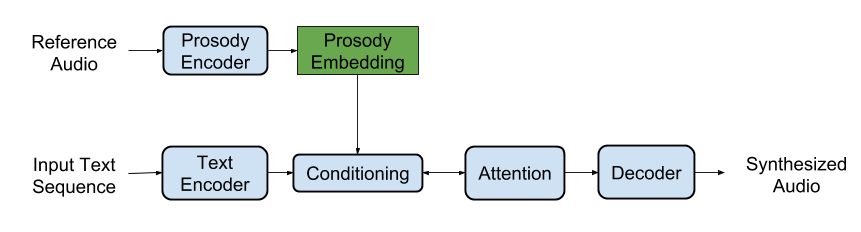
\includegraphics[width=0.75\textwidth]{figures/tacotron_prosody.png}
    \caption{Towards End-to-End Prosody Transfer for Expressive Speech Synthesis with Tacotron \cite{skerry2018towards}}
    \label{fig:tts}
\end{figure}

%%%%%%%%%%%%%%%%%%%%%%%%%%%%%%%%%%%%%%%%%%%%%%%%%%%%%%%%%%%%%%%%%%%%%%%%

%%%%%%%%%%%%%%%%%%%%%%%%%%%%%%%%%%%%%%%%%%%%%%%%%%%%%%%%%%%%%%%%%%%%%%%%
\subsection{Sample Efficient Adaptive Text-to-Speech}

There is growing interest in developing neural TTS models that can be trained end-to-end withoutthe need for hand-crafted representations.  In this study we focus on extending the autoregressiveWaveNet model (van den Oord et al., 2016; 2017) to the few-shot learning setting to adapt to speakersthat were not presented at training time. Other recent neural TTS models include Tacotron 2 (Skerry-Ryan et al., 2018) (building on (Wang et al., 2017)) which uses WaveNet as a vocoder to invertmel-spectrograms generated by an attentive sequence-to-sequence model. DeepVoice 2 (Gibianskyet al., 2017) (building on (Arık et al., 2017)) introduced a multi-speaker variation of Tacotron thatlearns a low-dimensional embedding for each speaker, which was further extended in DeepVoice 3(Ping et al., 2018) to a 2,400 multi-speaker scenario. Unlike WaveNet and DeepVoice, the Char2Wav(Sotelo et al., 2017) and VoiceLoop (Taigman et al., 2018) models produce World Vocoder Features(Morise et al., 2016) instead of generating raw audio signals.Although many of these systems have produced high-quality samples for speakers present in thetraining set, generalizing to new speakers given only a few seconds of audio remains a challenge.There have been several concurrent works to address this few-shot learning problem. The VoiceLoopmodel introduced a novel memory-based architecture that was extended by Nachmani et al. (2018)to few-shot voice style adaptation,  by introducing an auxiliary fitting network that predicts theembedding of a new speaker.  Jia et al. (2018) extended the Tacotron model for one-shot speakeradaptation by conditioning on a speaker embedding vector extracted from a pretrained speaker identitymodel of Wan et al. (2018). The most similar approached to our work was proposed by Arik et al.(2018) for the DeepVoice 3 model. They considered both predicting the embedding with an encodingnetwork and fitting the embedding based on a small amount of adaptation data, but the adaptationwas applied to a prediction model for mel-spectrograms with a fixed vocoder.

\cite{chen2018sample}
\footnote{\url{https://sample-efficient-adaptive-tts.github.io/demo/}}

%%%%%%%%%%%%%%%%%%%%%%%%%%%%%%%%%%%%%%%%%%%%%%%%%%%%%%%%%%%%%%%%%%%%%%%%
\section{Afweging en advies}
%%%%%%%%%%%%%%%%%%%%%%%%%%%%%%%%%%%%%%%%%%%%%%%%%%%%%%%%%%%%%%%%%%%%%%%%

Het aanpakken van een aantal facetten van Prosody.
\url{7700-transfer-learning-from-speaker-verification-to-multispeaker-text-to-speech-synthesis (1).pdf}